\documentclass[nogrid]{MBE}
\usepackage{url}

% Mol Biol Evol stuff
\jshort{mst}
\volname{}
\jvolume{0}
\jvol{}
\jissue{0}
\pubyear{2016}
\mstype{Article}
\artid{???}
\access{???}
\begin{document}

\title[Contact networks and ABC]{Phylodynamic inference of contact network
parameters through approximate Bayesian computation}
\author[McCloskey, Liang, and Poon]{Rosemary M. McCloskey$^{*,1}$, 
    Richard H. Liang$^1$, and Art F.Y. Poon$^{1,2}$}
\address{$^1$BC Centre for Excellence in HIV/AIDS, 608-1081 Burrard Street, Vancouver, Canada \\
$^2$Department of Medicine, University of British Columbia, Vancouver, Canada}
\history{Submitted 5 April 2016}
\coresp{E-mail: rmccloskey@cfenet.ubc.ca.}
\editor{}
\abstract{Models of the spread of disease in a population often make the simplifying
assumption that the population is homogeneously mixed, or is divided into
homogeneously mixed compartments. However, human populations have complex
structures formed by social contacts, which can have a significant influence on
the rate of epidemic spread. Contact network models capture this structure by
explicitly representing each contact that could possibly lead to a
transmission. We developed a method based on approximate Bayesian computation
(ABC) for estimating structural parameters of the contact network underlying an
observed viral phylogeny. The method combines adaptive sequential Monte Carlo
for ABC, Gillespie simulation for propagating epidemics though networks, and a
kernel-based tree similarity score. We used the method to fit the
Barab\'{a}si-Albert network model to simulated transmission trees and applied
it to viral phylogenies estimated from six real-world HIV sequence datasets. On
simulated data, we found that the preferential attachment power and the number
of infected nodes in the network can often be accurately estimated. On the
other hand, the mean degree of the network, as well as the total number of
nodes, appeared to be weakly or non-identifiable with ABC. We observed
substantial heterogeneity in the parameter estimates on real datasets, with
point estimates for the preferential attachment power ranging from 0.06 to
1.05. These results underscore the importance of considering contact structures
when performing phylodynamic inference. Our method offers the potential to
quantitatively investigate the contact network structure underlying viral
epidemics.
}
\keyword{Phylogenetics, phylodynamics, approximate Bayesian computation,
contact network, transmission tree, human immunodeficiency virus.}



\maketitle

\section{Introduction}

When an infectious disease spreads through a population, transmissions are
generally more likely to occur between certain pairs of individuals. Such pairs
must have a particular mode of contact with one another, which varies with the
mode of transmission of the disease. For airborne pathogens, physical proximity
may be sufficient, while for sexually transmitted diseases, \newpage\noindent %hack
sexual or in some cases blood-to-blood contact is required. The population
together with the set of links between individuals along which transmission can
occur is called the contact network~\citep{klovdahl1985social,
morris1993epidemiology}. The structure of the contact network underlying an
epidemic can profoundly impact the speed and pattern of the epidemic's
expansion. Network structure can influence the prevalence
trajectory~\citep{o2011contact} and epidemic
threshold~\citep{barthelemy2005dynamical}, in turn affecting the estimates of
quantities such as effective population size~\citep{goodreau2006assessing}.
From a public health perspective, contact networks have been explored as tools
for curtailing epidemic spread, by way of interventions targeted to
well-connected nodes~\citep{wang2015targeting}. True contact networks are a
challenging type of data to collect, requiring extensive epidemiological
investigation~\citep{welch2011statistical}.

Viral sequence data, on the other hand, has become relatively inexpensive and
straightforward to collect on a population level. Due to the high mutation rate
of RNA viruses, epidemiological processes impact the course of viral evolution,
thereby shaping the inter-host viral
phylogeny~\citep{drummond2003measurably}. The term ``phylodynamics'' was
coined to describe this interaction, as well as the growing family of inference
methods to estimate epidemiological parameters from viral
phylogenies~\citep{grenfell2004unifying}. These methods have revealed
diverse properties of local viral outbreaks, from basic reproductive
number~\citep{stadler2012estimating}, to the degree of
clustering~\citep{hughes2009molecular}, to the elevated transmission risk
during acute infection~\citep{volz2012simple}. On the other hand, although
sophisticated methods have been developed for fitting complex population
genetic models to phylogenies~\citep{rasmussen2014phylodynamic}, inference
of structural network parameters has to date been limited. However, it has been
shown that network structure has a tangible impact on phylogeny
shape~\citep{leventhal2012inferring, colijn2014phylogenetic,
goodreau2006assessing, robinson2013dynamics, villandre2016assessment},
suggesting that such statistical inference might be
possible~\citep{welch2011statistical}.

Survey-based studies of sexual networks~\citep{liljeros2001web,
schneeberger2004scale, colgate1989risk} have found that these networks tend to
have a degree distribution which follows a power law \citep[although there has
been some disagreement, see][]{handcock2004likelihood}. That is, the number of
nodes of degree $k$ is proportional to $k^{-\gamma}$ for some constant
$\gamma$. These networks are also referred to as ``scale-free''. One process by
which scale-free networks can be generated is preferential attachment, where
nodes with a high number of contacts attract new connections at an elevated
rate. The first contact network model incorporating preferential attachment was
introduced by \citet{barabasi1999emergence}, and is now referred to as the
Barab\'asi-Albert (BA) model. Under this model, networks are formed by
iteratively adding nodes with $m$ new edges each. In the most commonly studied
formulation, these new edges are joined to existing nodes of degree $k$ with
probability proportional to $k$, so that nodes of high degree tend to attract
more connections. \citeauthor{barabasi1999emergence} suggested an extension
where the probability of attaching to a node of degree $k$ is $k^\alpha$ for
some non-negative constant $\alpha$, and we use this extension here.

Previous work offers precedent for the possibility of statistical inference of
structural network parameters. \citet{britton2002bayesian} develop a Bayesian
approach to estimate the edge density in an Erd\H{o}s-R\'enyi
network~\citep{erdos1960evolution} given observed infection dates, and
optionally recovery dates. Their approach was later extended by
\citet{groendyke2011bayesian} and applied to a much larger data set of 188
individuals. \citet{volz2007susceptible, volz2008sir} developed differential
equations describing the spread of a susceptible-infected (SI) epidemic on
static and dynamic contact networks with several degree distributions, which
could in principle be used for inference if observed incidence trajectories
were available. \citet{brown2011transmission} analysed the degree distribution
of an approximate transmission network, estimated based on genetic similarity
and estimated times of infection, relating 60\% of HIV-infected men who have
sex with men (MSM) in the United Kingdom. The transmission network is a
subgraph of the contact network which includes only those edges which have
already led to a new infection. The authors found that a Waring distribution,
which is produced by a more sophisticated preferential attachment model, was a
good fit to their estimated network. 

Standard methods of model fitting involve calculation of the likelihood of
observed data under the model. In maximum likelihood estimation, a quantity
proportional to the likelihood is optimized, often through a standard
multi-dimensional numerical optimization procedure. Bayesian methods integrate
prior information by optimizing the posterior probability instead. To avoid
calculation of a normalizing constant, Bayesian inference is often performed
using Markov chain Monte Carlo (MCMC), which uses likelihood \emph{ratios} in
which the normalizing constants cancel out. Unfortunately, it is generally
difficult to explicitly calculate the likelihood of an observed transmission
tree under a contact network model, even up to a normalizing constant. To do
so, it would be necessary to integrate over all possible networks, and also
over all possible labellings of the internal nodes of the transmission tree.
While it is not known (to us) whether such integration is tractable, a simpler
alternative is offered by likelihood-free methods, namely approximate Bayesian
computation (ABC). ABC leverages the fact that, although calculating the
likelihood may be impractical, generating simulated datasets according to a
model is often straightforward. If our model fits the data well, the simulated
data it produces should be similar to the observed data. More formally, if $D$
is the observed data, the posterior distribution $f(\theta \mid D)$ on model
parameters $\theta$ is replaced as the target of statistical inference by
$f(\theta \mid \rho(\hat{D}, D) < \varepsilon)$, where $\rho$ is a distance
function, $\hat{D}$ is a simulated dataset according to $\theta$, and
$\varepsilon$ is a small tolerance~\citep{sunnaaker2013approximate}. In the
specific case when $\rho$ is a kernel function, the approach is known as
kernel-ABC~\citep{nakagome2013kernel, poon2015phylodynamic}.

Here, we develop a method using kernel-ABC to estimate the parameters of
contact network models from observed phylogenetic data. The distance function
we use is the tree kernel developed by \citet{poon2013mapping}, which computes
a weighted dot product of the trees' representations in the space of all
possible subset trees. We apply the method to investigate the parameters of the
BA network model on a variety of simulated and real datasets. Our results show
that some network parameters can be inferred with reasonable accuracy, while
others have a minimal detectable impact on tree shape and therefore cannot be
estimated accurately. We also find that these parameters can vary considerably
between real epidemics from different settings.

\section{New Approaches}

We have developed a kernel-ABC-based method to perform statistical inference of
contact network parameters from a transmission tree estimated from an observed
viral phylogeny. We implemented the adaptive sequential Monte Carlo (SMC)
algorithm for ABC developed by \citet{del2012adaptive}. The SMC algorithm keeps
track of a population of parameter ``particles'', which are initially sampled
from the parameters' joint prior distribution. Several datasets are simulated
under the model of interest for each of the particles. In this case, the
datasets are transmission trees, which are generated by a two-step process.
First, a contact network is simulated according to the network model being fit.
Second, a transmission tree is simulated over that network with a Gillespie
simulation algorithm~\citep{gillespie1976general}, in the same fashion as
several previous studies \citep[\textit{e.g.}][]{robinson2013dynamics,
leventhal2012inferring}. The particles are weighted according to the similarity
between their associated simulated trees and the observed tree. To quantify
this similarity, we used the tree kernel developed by \citet{poon2013mapping}.
Particles are iteratively perturbed by applying a Metropolis-Hastings kernel
and, if the move is accepted, simulating new datasets under the new parameters.
When a particle's weight drops to zero, because its simulated trees are too
dissimilar to the observed tree, the particle is dropped from the population,
and eventually replaced by a resampled particle with a higher weight. As the
algorithm progresses, the population converges to a Monte Carlo approximation
of the ABC target distribution, which is assumed to approximate the desired
posterior~\citep{del2012adaptive, sunnaaker2013approximate}.

A computer program implementing our method is freely available at
\url{https://github.com/rmcclosk/netabc} (last accessed April 3, 2016).

\section{Results}

\subsection{Kernel classifiers}



We investigated the parameters of the BA network
model~\citep{barabasi1999emergence}. In addition to $m$ and $\alpha$ (see
Introduction), we considered $N$, which denotes the total number of nodes in
the network, and $I$, which is the number of infected nodes at which to stop
the simulation and sample the transmission tree. To examine the effect of these
parameters on tree shape, we simulated transmission trees under different
parameter values, calculated pairwise tree kernel scores between them, and
attempted to classify the trees using a kernel support vector machine (kSVM).
We also tested classifiers based on Sackin's index~\citep{shao1990tree} and the
normalized lineages-through-time (nLTT)
statistic~\citep{janzen2015approximate}. Accuracy of the kSVMs varied based on
the parameter being tested (Figure~\ref{fig:rsquared}, left). Classifiers based
on two other tree statistics, the nLTT and Sackin's index, generally exhibited
worse performance than the tree kernel, although the magnitude of the disparity
varied between the parameters (Figure~\ref{fig:rsquared}, centre and right).
The results were largely robust to variations in the tree kernel
meta-parameters $\lambda$ and $\sigma$ (Figures~S3-S6).

When classifying $\alpha$, the kernel-SVM classifier had an average $R^2$ of 
    0.92,
compared to 
    0.56
for the nLTT-based SVM, and
    0.75
for the linear regression against Sackin's index. There was little variation
about the mean for different tree and epidemic sizes. No classifier could
accurately identify the $m$ parameter in any epidemic scenario, with average
$R^2$ values of 
  0.12 for kSVM,
  0.01 for the nLTT, and
  0.06
for Sackin's index. Again, there was little variation in accuracy between
epidemic scenarios, although the accuracy of the kSVM was slightly higher
on 1000-tip trees.

The accuracy of classifiers for $I$ varied significantly with the number of
tips in the tree. For 100-tip trees, the average $R^2$ values were
  0.7,
  0.55, and
  0.02
for the tree kernel, nLTT, and Sackin's index respectively. For 500-tip
trees, the values increased to
  0.93,
  0.83, and
  0.07.
Finally, the performance of classifiers for $N$ depended heavily on the
epidemic scenario. The $R^2$ of the kSVM classifier ranged from
  0.08
for the smallest epidemic and smallest sample size, to
  0.82
for the largest. Likewise, $R^2$ for the nLTT-based SVM ranged from 
  0.01
to
  0.54.
Sackin's index did not accurately classify $N$ in any scenario, with an average
$R^2$ of
  0.03
and little variation between scenarios.

\begin{figure*}[ht]
  \centering
  \includegraphics[width=\textwidth]{kernel-rsquared.eps}
  \vspace{6pt}
  \caption{
      Cross-validation accuracy of kernel-SVM classifier (left), SVM classifier
      using nLTT (centre), and linear regression using Sackin's index
      (right) for BA model parameters. Kernel meta-parameters were set to
      $\lambda = 0.3$ and $\sigma = 4$. Each point was calculated based on 300
      simulated transmission trees over networks with three different values of
      the parameter being tested. Vertical lines are empirical 95\% confidence
      intervals based on 1000 two-fold cross-validations.
  }
  \label{fig:rsquared}
\end{figure*}

\subsection{ABC simulations}



Figure~\ref{fig:abcpt} shows maximum \textit{a posteriori} (MAP) point
estimates of the BA model parameters obtained with kernel-ABC on simulated
data. The estimates shown correspond only to the simulations where the $m$
parameter was set to 2, however the results for $m = 3$ and $m = 4$ were
similar (Figures S7 and S8). Average boundaries of 95\% HPD intervals are given
in Table~\ref{tab:abchpd}.

The accuracy of the parameter estimates obtained with kernel-ABC
paralleled the results from the kSVM classifier. Of the four parameters,
$\alpha$ was the most accurately estimated, with point estimates having a
median [IQR] absolute error of 
    0.11 
    [0.05 - 
    0.18].
The errors when the true value of $\alpha$ was zero were significantly greater
than those for the other values 
    (Wilcoxon rank-sum test, $p$ = $6\!\times\!10^{-4}$),
but did not vary across the true values of the other parameters (one-way
ANOVA). Estimates for $I$ were also relatively accurate, with point estimate
errors of
    306 
    [108 - 
    607].
These errors were significantly higher when the true value of $\alpha$ was
at least 1
    (Wilcoxon rank-sum test, $p$ = $6\!\times\!10^{-4}$)
and when the true value of $I$ was 2000 ($p < 10^{-5}$). The true value of $m$
did not affect the estimates of $I$ (one-way ANOVA).

The $m$ parameter was estimated correctly in only
    37 \%
of simulations. Oddly, the error in the estimated $m$ was higher for integer
values of $\alpha$ (\text{i.e.}~0 and 1) than non-integer values 
    (Wilcoxon rank-sum test, $p$ = 0.007).
The true values of the other parameters did not significantly affect the
estimates of $m$ (both one-way ANOVA). Finally, the total number of nodes $N$
was consistently over-estimated by about a factor of two
    (error 6588 
    [4214 - 
     8284]).
No parameters influenced the accuracy of the $N$ estimates (all one-way ANOVA).

\begin{figure*}[ht]
  \centering
  \includegraphics[width=\textwidth]{abc-point-estimate-m2.eps}
  \vspace{6pt}
  \caption{
    Point estimates of BA model parameters obtained by running kernel-ABC
    on simulated phylogenies without training, for simulations with $m = 2$.
    Dotted lines indicate true values, and limits of the $y$-axes are regions
    of uniform prior density. (A) Estimates for $\alpha$ and $I$ against their
    true values in simulations. (B) Estimates for $m$ and $N$, which were held
    fixed in these simulations, against true values of $\alpha$.
  }
  \label{fig:abcpt}
\end{figure*}

\begin{table*}[ht]
  \centering
    \begin{tabular}{lr>{\raggedleft\arraybackslash}p{2.5cm}>{\raggedleft\arraybackslash}p{2.5cm}>{\raggedleft\arraybackslash}p{2.5cm}}
      \hline
    Parameter & True value & Mean point estimate & Mean HPD lower bound & Mean HPD upper bound \\ 
      \hline
    $\alpha$ & 0.0 & 0.24 & 0.02 & 0.73 \\ 
       & 0.5 & 0.42 & 0.02 & 0.81 \\ 
       & 1.0 & 0.97 & 0.61 & 1.11 \\ 
       & 1.5 & 1.48 & 1.26 & 1.83 \\ 
      $I$ & 1000 & 1155.68 & 598.68 & 2402.84 \\ 
       & 2000 & 2646.07 & 1182.31 & 4058.13 \\ 
      $m$ & 2 & 2.92 & 1.75 & 4.92 \\ 
       & 3 & 3.33 & 1.96 & 4.92 \\ 
       & 4 & 3.62 & 1.88 & 5.00 \\ 
      $N$ & 5000 & 10962.61 & 2732.55 & 14701.87 \\ 
       \hline
    \end{tabular}
  \caption{
      Average maximum \textit{a posteriori} point estimates and 95\% highest
      posterior density (HPD) interval widths for BA model parameter estimates
      obtained with kernel-ABC. Three transmission trees were simulated under
      each combination of the listed parameter values, and the parameters were
      estimated with kernel-ABC without training.
  }
  \label{tab:abchpd}
\end{table*}

The dispersion of the ABC approximation to the posterior also varied between
the parameters, with narrower HPD intervals for the parameters with more
accurate point estimates (Table~\ref{tab:abchpd}). Figure~\ref{fig:abcex} shows
the distributions for for one simulation (equivalent plots for all the
simulations can be found in Supplementary Figure S10). HPD intervals around $\alpha$
and $I$ were narrow relative to the region of nonzero prior density, whereas
the intervals for $m$ and $N$ were more widely dispersed.

\begin{figure*}[ht]
    \centering
  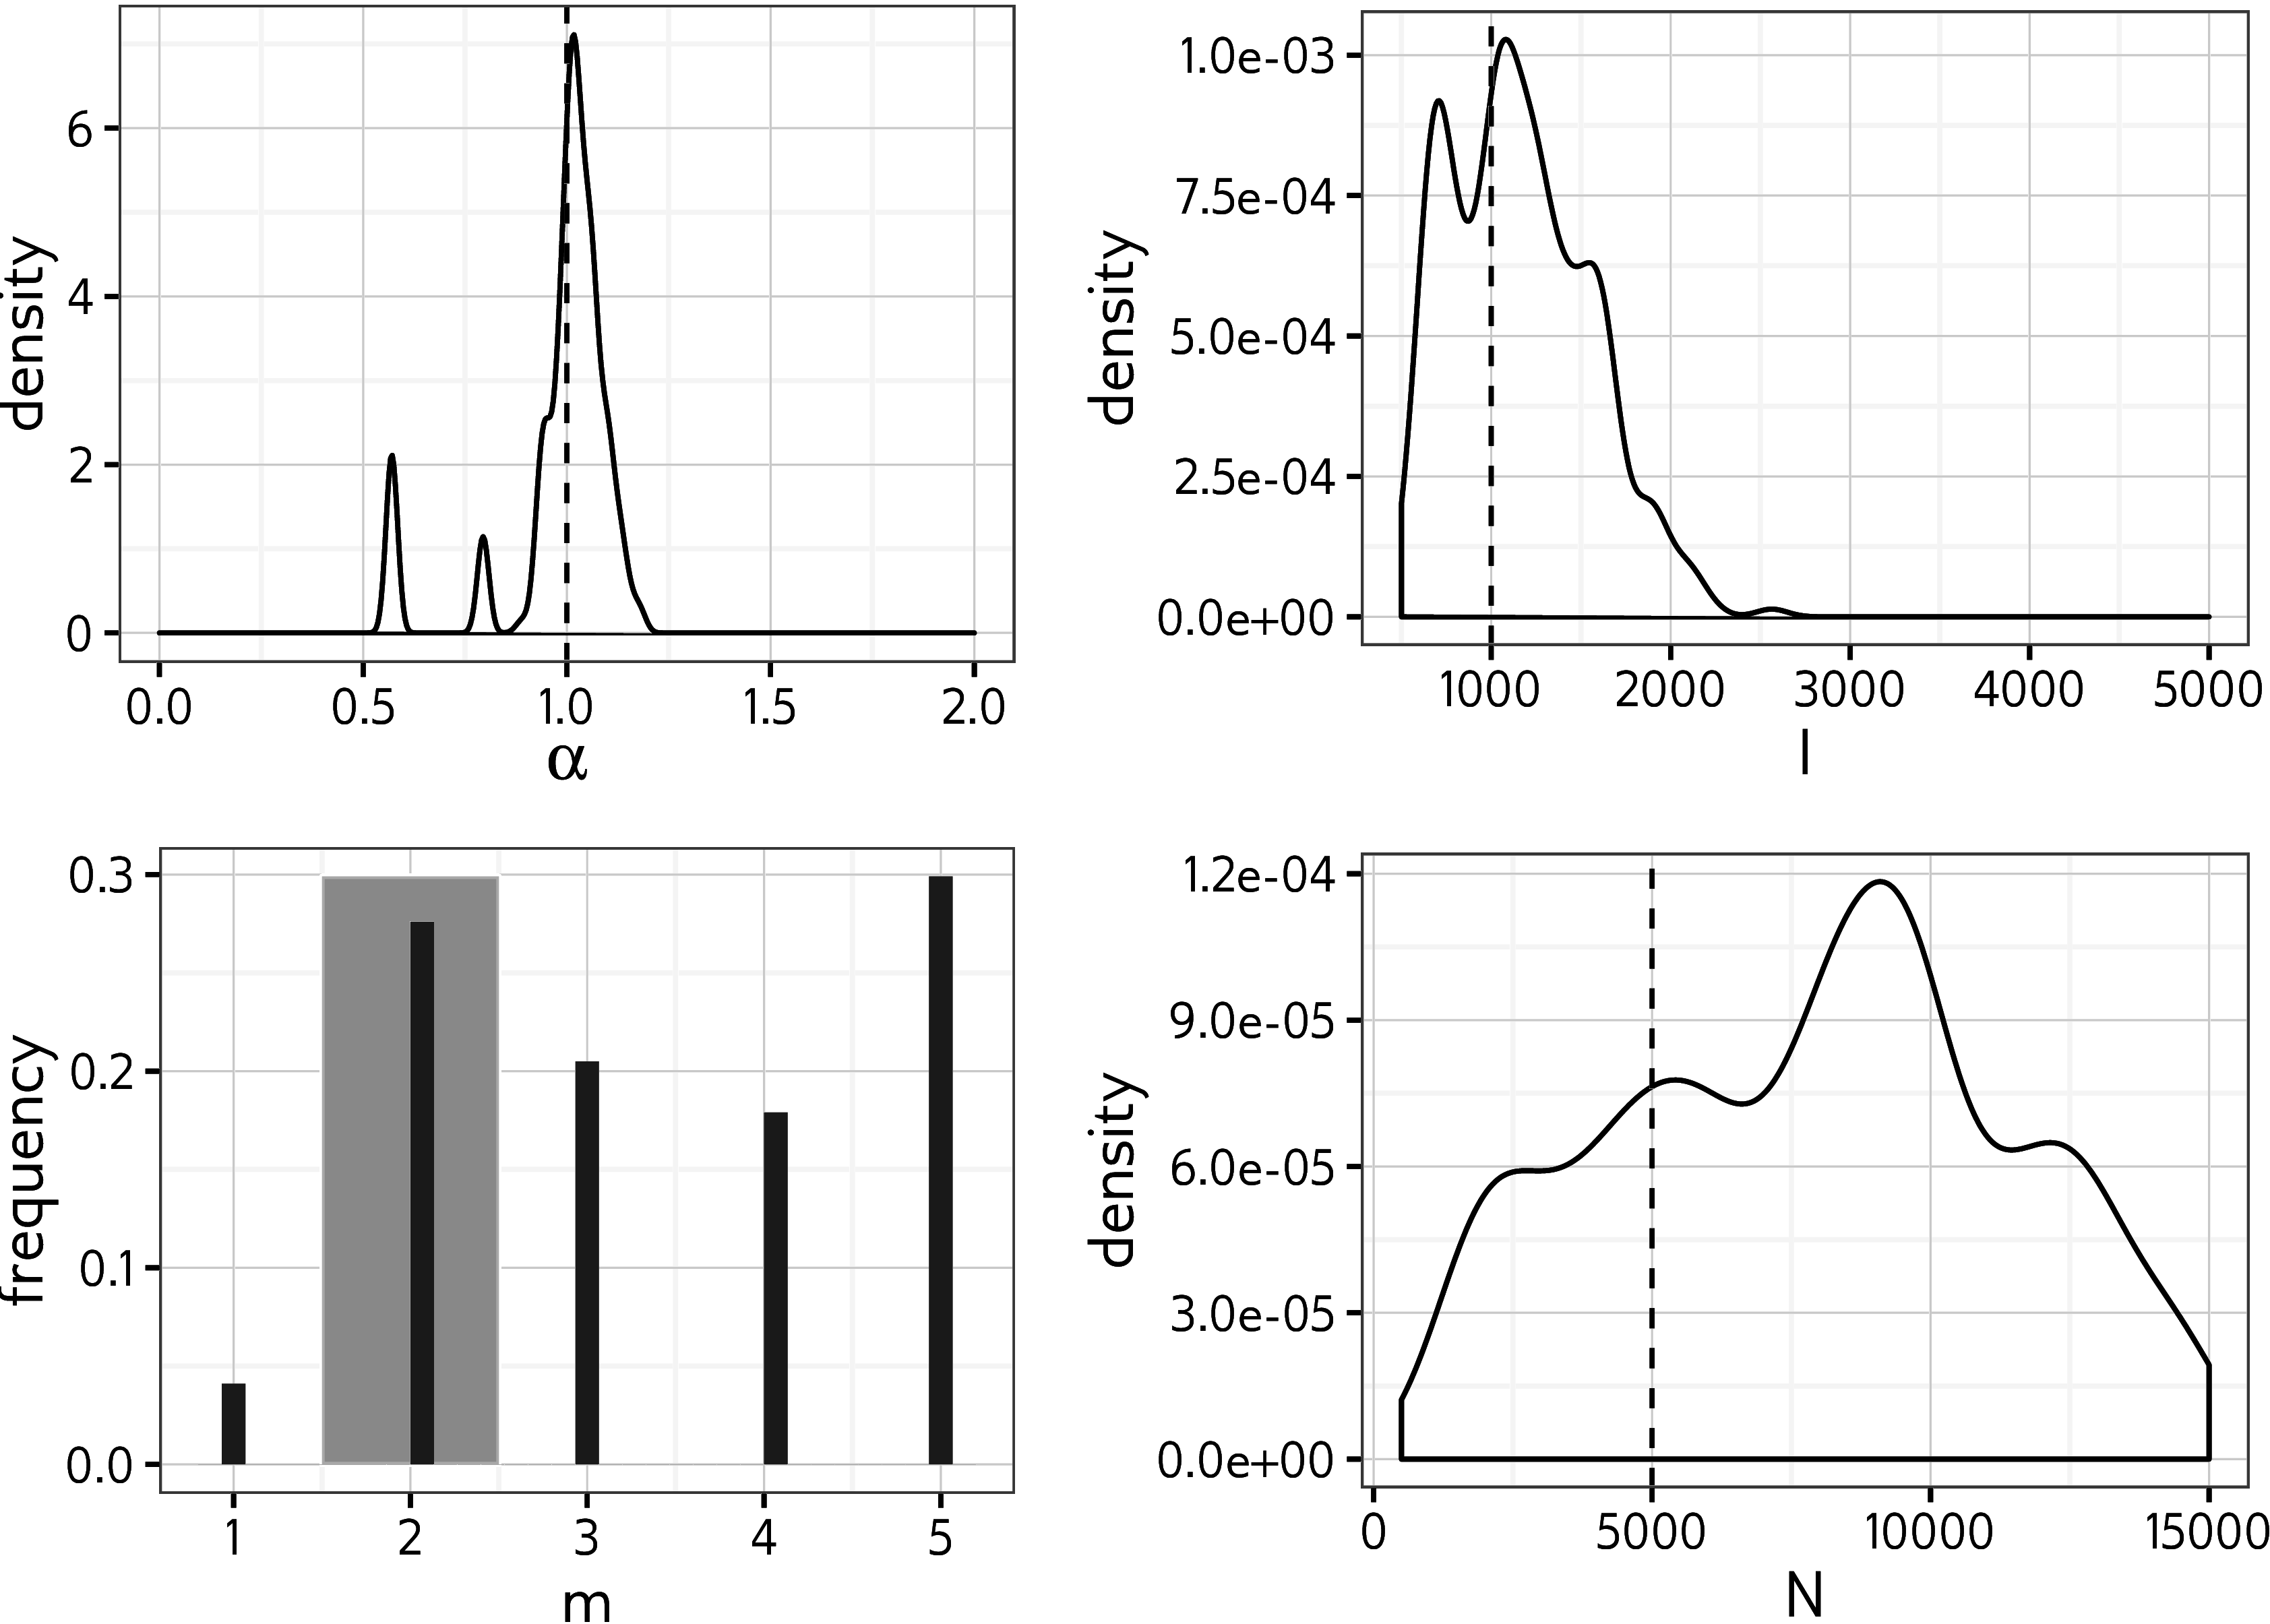
\includegraphics[width=\textwidth]{abc-posterior-example.eps}
  \vspace{6pt}
  \caption{
    Marginal posterior distributions of BA model parameters estimated
    with kernel-ABC for a single simulated transmission tree. Dotted
    lines and shaded polygon indicate true values.
  }
  \label{fig:abcex}
\end{figure*}



To test the effect of model misspecification, we simulated one network where
the nodes exhibited heterogeneous preferential attachment power (half 0.5, the
other half 1.5), with $m$ = 2, $N$ = 5000, and $I$ = 1000. The MAP [95\%
HPD] estimates for each parameter were: 
$\alpha$, 
  1 
  [0.07-
   1.07];
$I$,
  1170 
  [506 -
   1616];
$m$,
  5 
  [2 -
   5];
$N$,
  \ensuremath{1.033\times 10^{4}} 
  [2408-
   \ensuremath{1.4974\times 10^{4}}].
To test the effect of sampling bias, we sampled one transmission tree in a
peer-driven fashion, where the probability to sample a node was twice as high
if one of its peers had already been sampled. The parameters for this
experiment were $N$ = 5000, $m$ = 2, $\alpha$ = 0.5, and $I$ = 2000. The
estimated values were
$\alpha$, 
  0.48 
  [0.03 -
   0.82];
$I$,
  2468 
  [1281 -
   3938];
$m$,
  3 
  [2 -
   5];
$N$,
  \ensuremath{1.0738\times 10^{4}} 
  [3106 -
   \ensuremath{1.4783\times 10^{4}}].
Both of these results were in line with estimates obtained on other simulated
datasets (Table~\ref{tab:abchpd}).

\subsection{Real data}



We applied kernel-ABC to five published HIV datasets (Table~\ref{tab:data}),
and found substantial heterogeneity among the parameter estimates
(Figure~\ref{fig:abchpd}). Two of the datasets~\citep{niculescu2015recent,
wang2015targeting} had estimated $\alpha$ values near unity (MAP estimates
[95\% HPD] 
  1.06 
  [0.63 - 
   1.27]
and
  1 
  [0.41 -
   1.16] respectively). 
Another two datasets~\citep{li2015hiv, cuevas2009hiv} had lower estimated
values and wider HPD intervals
  (0.77 
  [0.01 - 
  1.03]
and
  0.66 
  [0.03 -
   0.84]). 
The \citet{novitsky2014impact} data had an extremely low estimated $\alpha$
and a very wide HPD interval
  (0.17 
  [0.04 -
   1.39]). 
For all the datasets except \citeauthor{novitsky2014impact}, estimated values of
$I$ were below 2000, with narrow HPD intervals around two of the
datasets
  (\citeauthor{cuevas2009hiv}, 880 
  [290 -
   1511];
   \citeauthor{niculescu2015recent}, 175
  [138 - 
   454])
and wider intervals around the other two
  (\citeauthor{li2015hiv}, 1590 
  [284 -
   3807];
   \citeauthor{wang2015targeting}, 651
  [268 - 
   4235]).
The \citeauthor{novitsky2014impact} data was again the outlier, with a very high
estimated $I$, and HPD interval spanning almost the entire prior region
  (7547 
  [228 -
   8921]).
No information was gleaned about the $m$ parameter, with the HPD interval
occupying the entire prior region for all datasets. The estimates of $N$ were
similarly uninformative, with the exception that the point estimate for the
\citeauthor{wang2015targeting} data was smaller
  (5839)
than the estimates for other datasets
 (average 8927).

\begin{figure*}[ht]
  \centering
  \includegraphics{realdata-hpd.eps}
  \vspace{8pt}
  \caption{
      Maximum \textit{a posteriori} point estimates and 95\% HPD intervals for
      parameters of the BA network model, fitted to five published HIV datasets
      with kernel-ABC.
  }
  \label{fig:abchpd}
\end{figure*}

\section{Discussion}

Contact networks can have a strong influence on epidemic progression, and are
potentially useful as a public health tool~\citep{wang2015targeting,
little2014using}. Despite this, few methods exist for investigating contact
network parameters in a phylodynamic framework~\citep{groendyke2011bayesian,
volz2008sir, brown2011transmission, leventhal2012inferring}. Kernel-ABC is a
model-agnostic method which can be used to investigate any quantity that
affects tree shape~\citep{poon2015phylodynamic}. In this work, we developed a
kernel-ABC-based method to infer the parameters of a contact network model. The
method is general, and could be applied to any model from which contact
networks can be simulated. We demonstrated the method on the BA model,
which is a simple preferential attachment model giving rise to the power law
degree distributions commonly observed in real-world networks. 

By training a kernel-SVM classifier, we found that the $\alpha$ and $I$
parameters, representing preferential attachment power and number of infected
nodes, had a strong influence on tree shape. This was reflected in the relative
accuracy of the kernel-ABC estimates of these parameters. The total number of
nodes $N$ had a weak influence on tree shape, which was most prominent when the
epidemic size $I$ and number of sampled tips were both large. The $m$
parameter, representing the number of edges created in the network per vertex,
did not produce much variation in tree shape, resulting in in both poorly
performing classifiers and uninformative kernel-ABC estimates.

$N$ was almost always significantly over-estimated using kernel-ABC. Since the
prior on $N$ and $I$ is jointly uniform on a non-rectangular region ($I \leq
N$), there is more prior mass on high $N$ values. In retrospect, it is
unreasonable to expect good estimation of $N$, because adding more nodes to a
BA network does not change the edge density or overall shape. This can be
illustrated by imagining that we add a small number of nodes to a network after
the epidemic simulation has already been completed. It is possible that none of
these new nodes attains a connection to any infected node. Thus, running the
simulation again on the new, larger network could produce the exact same
transmission tree as before. 

As noted by \citet{lintusaari2016identifiability}, uniform priors on model
parameters may translate to highly informative priors on quantities of
interest. We observed a non-linear relationship between the preferential
attachment power $\alpha$ and the power law exponent $\gamma$ (Figure~S9).
Therefore, placing a uniform prior on $\alpha$ between 0 and 2 is equivalent to
placing an informative prior that $\gamma$ is close to 2. Therefore, if we were
primarily interested in $\gamma$ rather than $\alpha$, a more sensible choice
of prior might have a shape similar to the inverse of Figure~S9 and be bounded
above by approximately $\alpha$ = 1.5. This would uniformly bound $\gamma$ in
the region $2 \leq \gamma \leq 4$ commonly reported in the network
literature~\citep{liljeros2001web, schneeberger2004scale, colgate1989risk,
brown2011transmission}. We note however that \citet{jones2003assessment}
estimated $\gamma$ values greater than four, in one case as high as 17, for
some datasets, indicating that a wider range of permitted $\gamma$ values may
be warranted.

Our investigation of published HIV datasets indicated heterogeneity in the
contact network structures underlying several distinct local epidemics. The
five datasets analysed fell into three categories (Figure~\ref{fig:abchpd}).
First, we estimated a preferential attachment power between 0.5 and 1 for the
epidemics studied by \citet{cuevas2009hiv} and \citet{li2015hiv}, with credible
intervals occupying nearly the entire region from 0 to 1.
\citeauthor{cuevas2009hiv} studied a group of newly diagnosed individuals in
the Basque Country, Spain. Although the individuals were of mixed risk groups,
and therefore unlikely to comprise a single contact network, a high proportion
of them (47\%) grouped into local clusters based on genetic distance. The low
estimated attachment power for these data is consistent with the sampled
sequences comprising many distinct sub-networks rather than a single connected
network. \citeauthor{li2015hiv} sampled a large number of acutely infected
MSM in Shanghai, China, in which we identified a large cluster from the
phylogeny using a patristic distance cutoff~\citep{poon2015impact}. The low
attachment power estimated for this dataset was surprising given the high
phylogenetic relatedness of the sequences. It is possible that the number and
diversity of circulating recombinant forms in the data introduced errors into
our estimated viral phylogeny.

For the outbreaks studied by \citet{niculescu2015recent} and
\citet{wang2015targeting}, the estimated $\alpha$ was close to one, with a
narrower credible interval than for the other studies.
\citeauthor{niculescu2015recent} studied a recent outbreak among Romanian
injection drug users (IDU), while \citeauthor{wang2015targeting} sampled
acutely infected MSM in Beijing, China. Both studies discovered a high degree
of phylogenetic relatedness owing to the recent infection times and homogeneous
risk groups of the studied populations. The estimated number of infections for
these datasets were also quite low, although the HPD interval for
\citeauthor{wang2015targeting} was much wider than that for
\citeauthor{niculescu2015recent}.

The final studied dataset was an outlier in terms of estimated parameters.
\citet{novitsky2013phylogenetic} sampled approximately 44\% of the
HIV-infected individuals in the northern area of Mochudi, Botswana. Additional
sampling in a later study~\citep{novitsky2014impact} brought the genotyping
coverage up to 70\%. Even with such a high sampling coverage, we did not detect
any large clusters using patristic distance, and therefore chose to analyze a
subtree instead. Estimates of $\alpha$ and $N$ both had very wide HPD
intervals and were markedly different from the other datasets. The estimated
number of infected nodes was also extremely high, much higher than the
estimated HIV prevalence of the town. Several factors may have contributed to
these results. First, the authors note that the their sample was 75\% female.
In a primarily heterosexual risk environment, removal of a disproportionate
number of males from the network could obfuscate the true network structure,
for example if the majority of highly connected nodes were of one gender.
Second, the town in question was in close proximity to the country's capital,
and the authors indicated that a high amount of migration takes place between
the two locations. This suggests that the contact network may include a much
larger group based in the capital city, which would explain the high estimate
of $I$.

When interpreting these results, we caution that the BA model is quite
simple and most likely misspecified for these data. In particular, the average
degree of a node in the network is equal to $2m$, and therefore is constrained
to be a multiple of 2. Furthermore, we considered the case $m = 1$, where the
network has no cycles, to be implausible and assigned it zero prior
probability. This forces the average degree to be at least four, which may be
unrealistically high for sexual networks. Additional modelling assumptions
include the network being connected and static, all transmission rates being
equal, no removal after infection, and identical behaviour of all nodes. This
last is particularly problematic, as we showed by simulating a network where
some nodes exhibited a higher attachment power than others. The estimated
attachment power was simply the average of the two values, indicating that,
although we could characterize the network in aggregate, the estimated
parameters could not be said to apply to any individual node. Despite these
issues, we felt it was best to demonstrate the method first on a simple model.
It is possible to use this framework to fit more complex models which address
some of these issues, such as one incorporating heterogeneous node behaviour,
which may prove a fruitful avenue for future investigations.

Our method has a number of caveats, perhaps the most significant being that it
takes a transmission tree as input. In reality, true transmission trees are not
available and must be approximated, often by way of a viral phylogeny. Although
this has been demonstrated to be a fair
approximation~\citep[e.g.][]{leitner1996accurate}, and is frequently used in
practice~\citep[e.g.][]{stadler2013uncovering}, the topologies of a viral
phylogeny and transmission tree can differ
significantly~\citep{ypma2013relating} due to within-host evolution and the
sampling process. In addition, the ABC-SMC algorithm is
computationally intensive, taking about a day when run on 20 cores in parallel
with the settings we described in the methods. Nevertheless, our method is
potentially useful to epidemiological researchers interested in the general
characteristics of the network structure underlying disease outbreaks. This
work, and previous work by our group~\citep{poon2015phylodynamic}, has
demonstrated that kernel-ABC is a broadly applicable and effective framework in
which to perform phylodynamic inference.

\section{Materials and Methods}
  
Nodes in our networks followed simple SI dynamics, meaning that they
became infected at a rate proportional to their number of infected neighbours,
and never recovered. For all analyses, the transmission trees' branch lengths
were scaled by dividing by their mean. We used the \textit{igraph} library's
implementation of the BA model~\citep{csardi2006igraph} to generate the graphs.
The analyses were run on Westgrid (\url{https://www.westgrid.ca/}) and a local
computer cluster.

\subsection{Computer program validation}

To check that our implementation of Gillespie simulation was correct, we
reproduced Figure 1A of \citet{leventhal2012inferring} (our Figure~S1), which
plots the unbalancedness of transmission trees simulated over four network
models at various levels of pathogen transmissibility. Our implementation of
adaptive ABC-SMC was tested by applying it to the same mixture of Gaussians
used by \citeauthor{del2012adaptive} to demonstrate their method (originally
used by~\citet{sisson2007sequential}). We were able to obtain a close
approximation to the function (see Figure~S2), and attained the stopping
condition used by the authors in a comparable number of steps. 

\subsection{Kernel classifiers}
  
We used the phylogenetic kernel developed by \citet{poon2013mapping} to test
whether the parameters of the BA model had an effect on tree shape. 100
networks were simulated under each of three different values of $\alpha$: 0.5,
1.0, and 1.5 (300 networks total). The other parameters were fixed to the
following values: $N$ = 5000, $I$ = 1000, and $m$ = 2. A transmission tree with
500 tips was simulated over each network (300 transmission trees total). The
300 trees were compared pairwise with the tree kernel to form a $300 \times
300$ kernel matrix. The kernel meta-parameters $\lambda$ (the ``decay
factor''), and $\sigma$ (the ``radial basis function
variance'')~\citep[see][]{poon2013mapping}, were set to 0.3 and 4 respectively.
We constructed a kSVM classifier for $\alpha$ using the \textit{kernlab}
package~\citep{zeileis2004kernlab}, and evaluated its accuracy with 1000
two-fold cross-validations.
  
Three similar experiments were performed for the other BA model parameters (one
experiment per parameter). $m$ was varied between 2, 3, and 4; $I$ between 500,
1000, and 2000; and $N$ between 3000, 5000, and 8000. The parameters not being
tested were fixed at the values $N$ = 5000, $I$ = 1000, $m$ = 2, and $\alpha$ =
1. Thus, we performed a total of four kSVM cross-validations, one for each of
the BA model parameters $\alpha$, $I$, $m$, and $N$. We repeated these four
cross-validations with different values of $\lambda$ (0.2, 0.3, and 0.4) and
$\sigma$ ($2^{-3}$, $2^{-2}$, \ldots, $2^3$), as well as on trees with
differing numbers of tips (100, 500, and 1000) and in epidemics of differing
size (500, 1000, and 2000). The combination of the number of sampled
individuals (\textit{i.e.} the number of tips) and the epidemic size
(\textit{i.e.} $I$) will be referred to as an ``epidemic scenario''. When
evaluating the classifier for $I$, we did not consider trees with 1000 tips,
because one of the tested $I$ values was 500, and the number of tips cannot be
larger than $I$.
  
For each of the four parameters, we also tested a linear regression against
Sackin's index~\citep{shao1990tree} and an ordinary SVM based on the normalized
lineages-through-time (nLTT) statistic~\citep{janzen2015approximate}.
  
\subsection{ABC simulations}
  
We simulated three transmission trees, each with 500 tips, under every element
of the Cartesian product of these parameter values: $N$ = 5000, $I$ =
\{1000, 2000\}, $m$ = \{2, 3, 4\}, and $\alpha$ = \{0.0, 0.5, 1,
1.5\}. This produced a total of 24 parameter combinations $\times$ three trees
per combination = 72 trees total. The adaptive ABC algorithm was applied to
each tree with these priors: $m \sim$ Uniform(1, 5), $\alpha \sim$ Uniform(0,
2), and $(N, I)$ jointly uniform on the region \{$500 \leq N \leq 15000$, $500
\leq I \leq 5000$, $I \leq N$\}. Following \citet{del2012adaptive} and
\citet{beaumont2009adaptive}, all proposals were Gaussian, with variance equal
to twice the empirical variance of the particles. The algorithm was run with
1000 particles, 5 simulated datasets per particle, and the ``quality''
parameter controlling the decay rate of the tolerance $\varepsilon$ set to
0.95. We used the same stopping criterion as \citeauthor{del2012adaptive},
namely when the MCMC acceptance rate dropped below 1.5\%. Point estimates for
the parameters were obtained by taking the highest point of an estimated kernel
density on the final set of particles, calculated using the \textit{density}
function with the default parameters in \textit{R}. Highest posterior density
(HPD) intervals were calculated with the \textit{HPDinterval} function from
the \textit{R} package \textit{coda}~\citep{plummer2006coda}.
  
Two further analyses were performed to address potential sources of error. To
evaluate the effect of model misspecification in the case of heterogeneity
among nodes, we generated a network where half the nodes were attached with
power $\alpha$ = 0.5, and the other half with power $\alpha$ = 1.5. The other
parameters for this network were $N$ = 5000, $I$ = 1000, and $m$ = 2. To
investigate the effects of potential sampling bias, we simulated a transmission
tree where the tips were sampled in a peer-driven fashion, rather than at
random. That is, the probability to sample a node was twice as high if any of
that node's network peers had already been sampled. The parameters of this
network were $N$ = 5000, $I$ = 2000, $m$ = 2, and $\alpha$ = 0.5.
  
\subsection{Investigation of published data}
  
We applied our kernel-ABC method to several published HIV datasets. Because the
BA model generates networks with a single connected component, we
specifically searched for datasets which originated from existing clusters,
either phylogenetically or geographically defined. Characteristics of the
datasets we investigated are given in Table~\ref{tab:data}.
  
\begin{table*}[!t]
  \centering
  \begin{tabular}{ccccc}
    Reference & Sequences ($n$) & Location & Risk group & Gene \\
    \hline
    \citet{wang2015targeting} & 173 & Beijing, China & MSM & \textit{pol} \\
    \citet{cuevas2009hiv} & 287 & Basque Country, Spain & mixed & \textit{pol} \\
    \citet{novitsky2013phylogenetic} & \multirow{2}{*}{180} &
    \multirow{2}{*}{Mochudi, Botswana} & \multirow{2}{*}{mixed} &
    \multirow{2}{*}{\textit{env}} \\ \citet{novitsky2014impact} \\
    \citet{li2015hiv} & 280 & Shanghai, China & MSM & \textit{pol} \\
    \citet{niculescu2015recent} & 136 & Romaina & IDU & \textit{pol} \\
    \hline
  \end{tabular}
  \caption{Characteristics of published datasets investigated with kernel-ABC.
  Acronyms: MSM, men who have sex with men; IDU, injection drug users.}
  \label{tab:data}
\end{table*}

We downloaded all sequences associated with each study from GenBank. For the
\citet{novitsky2014impact} data, each sequence was aligned pairwise to the HXB2
reference sequence (Genbank accession number K03455) and the hypervariable
regions were clipped out with \textit{BioPython} version
1.66+~\citep{cock2009biopython}. Sequences were multiply aligned using
\textit{MUSCLE} version 3.8.31 \citep{edgar2004muscle}, and alignments were
manually inspected with \textit{Seaview} version 4.4.2
\citep{gouy2010seaview}. Phylogenies were constructed from the nucleotide
alignments by approximate maximum likelihood using \textit{FastTree2} version
2.1.7 with the generalized time-reversible model. Transmission trees were
estimated by rooting and time-scaling the phylogenies by root-to-tip
regression, using a modified version of Path-O-Gen (distributed as part of
BEAST~\citep{drummond2007beast}) as described
previously~\citep{poon2015phylodynamic}. 

Two of the datasets \citep{li2015hiv,novitsky2014impact} were initially much
larger than the others, containing 1265 and 1299 sequences respectively. To
ensure that the analyses were comparable, we reduced these to a number of
sequences similar to the smaller datasets. For the \citet{li2015hiv} data,
we detected a cluster of size 280 using a patristic distance cutoff of 0.02 as
described previously~\citep{poon2015impact}. Only sequences within this
cluster were carried forward. For the \citet{novitsky2014impact} data, no
large clusters were detected using the same cutoff, so we analysed a subtree of
size 180 chosen arbitrarily.

For all datasets, we used the priors $\alpha$ $\sim$ Uniform(0, 2), $m$ $\sim$
Uniform(2, 5), and $N$ and $I$ jointly uniform on the region 
\{$n \leq N \leq 10000$, $n \leq I \leq 10000$, $I \leq N$\}, where $n$ is the
number of tips in the tree. The other parameters to the SMC algorithm
were the same as used for the simulation experiments.

\section{Supplementary data}

Supplementary figures S1-S10 are available at Molecular Biology and Evolution
online (\url{http://www.mbe.oxfordjournals.org/}).

\section{Acknowledgements}

This work was supported by grants from the Canadian Institutes of Health
Research (CIHR, operating grant HOP-111406), and the Bill \& Melinda Gates
Foundation (award number OPP1110049). R.M.M. was supported by a scholarship
from the CIHR Strategic Training Program in Bioinformatics. A.F.Y.P. was
supported by a CIHR New Investigator Award (Canadian HIV Vaccine Initiative,
Vaccine Discovery and Social Research) and by a Career Investigator Scholar
Award from the Michael Smith Foundation for Health Research, in partnership
with the Providence Health Care Research Institute and St. Paul's Hospital
Foundation.

\bibliographystyle{natbib}
\bibliography{papers}

\end{document}
